\section{The Dactylopiidae}
The Dactylopiidae family (Hemiptera: Sternorrhyncha: Coccoidea) comprises 11 species and a variety of intraspecific lineages in the \textit{Dactylopius} genus; which are all indigenous to the Americas \citep{Rodriguez2001, VanDam2012} (Table \ref{tab:dactylopius_species}). 

\vspace{0.5cm}

\begin{table}[H]
\caption{A list of the 11 recorded \textit{Dactylopius} species and intraspecific lineages} \label{tab:dactylopius_species}
\centering
\renewcommand{\arraystretch}{0.5}
\begin{tabular}{@{}l@{}}
\toprule
\multicolumn{1}{c}{Species} \\ \midrule
\textit{Dactylopius austrinus} De Lotto \\
\textit{Dactylopius bassi} Targioni Tozzetti \\
\textit{Dactylopius ceylonicus} Green \\
\textit{Dactylopius coccus} Costa \\
\textit{Dactylopius confertus} De Lotto \\
\textit{Dactylopius confusus} Cockerell \\
\textit{Dactylopius gracilipilus} Van Dam \& May \\
\begin{tabular}[c]{@{}l@{}}\textit{Dactylopius opuntiae} Cockerell\\ Lineages: `ficus', and `stricta' \end{tabular} \\
\begin{tabular}[c]{@{}l@{}}\textit{Dactylopius tomentosus} Lamarck\\ Lineages: `bigelovii', `californica var. parkeri', \\ `cholla', `cylindropuntia sp.', `echinocarpa x \\ acanthocarpa', `imbricata' \end{tabular} \\
\textit{Dactylopius salmianus} De Lotto \\
\textit{Dactylopius zimmermannii} De Lotto \\ \bottomrule
\end{tabular}
\end{table}

\noindent  Four of these are currently used as biological control agents in South Africa and Australia; namely \textit{D. austrinus} De Lotto, \textit{D. ceylonicus} Green, \textit{D. opuntiae} Cockerell, and \textit{D. tomentosus} Lamarck \citep{DeLotto1974, Perez-Guerra1992, managingOpuntioid2017}. 
% These sap-sucking insects feed predominantly on cactaceous plants in the \textit{Opuntia} and \textit{Nopalea} genera \citep{DeLotto1974, VanDam2012, Campana2015}. 
All species produce carminic acid, a deep red anthraquinone, as a defensive compound \citep{Eisner1980, Perez-Guerra1992}. The Aztecs and Incas domesticated \textit{D. coccus} as a dye for wool, cotton, paint, and cosmetics \citep{Nobel2002CactiUses}. The dye has been used for over two thousand years, with the first historical reports from Peru dating back to the early 1500s \citep{Nobel2002CactiUses}. The Spanish conquistadors initiated large-scale cultivation of the insects in Oaxaca, Mexico, and began exporting them to Europe by the year 1526 \citep{Meyer2000}. The dye became the third highest source of income to the Spanish Empire after gold and silver \citep{Humboldt1966,Chavez-Moreno2009TheDistribution}.

\subsection{Identification issues}
The taxonomy of the Dactylopiidae is largely understudied, and until fairly recently, only morphological characters were used to create phylogenies \citep{Ramirez-Puebla2010MolecularBacteria}. The history of this insect's taxonomy is rooted in misidentifications. Many of the species are notoriously difficult to differentiate using morphological traits, even for experts \citep{Mann1969Cactus-feedingMites, Perez-Guerra1992, Gullan1997, Portillo2006AENEMIES}. Considering the high species diversity of the Cactaceae, the probability of there being many more \textit{Dactylopius} species, cryptic species, and lineages in the native range is very high. Using molecular tools to assist in the taxonomic organisation of this group is therefore very valuable. Different \textit{Dactylopius} species and lineages display different levels of damage on target Cactaceae, and so correctly distinguishing between them is fundamental to selecting the most effective agents for biological control programmes. This is where the use of genetic barcoding can be useful. 

\subsection{`Biotypes'}
\label{sec:biotypes}

Species within the Dactylopiidae consist of genetically and/or behaviourally-distinct groups, which have been referred to as `biotypes' in the literature \citep{githure1999host, Volchansky1999, Hoffmann2004a, Mathenge2009, Mathenge2010a, Mathenge2010, Jones2015, Mathenge2015}. \citet{Mathenge2010}, for example, suggest that \textit{``biotypes of} Dactylopius \textit{species may not have developed sufficient behavioural, physiological or genetic changes during their prolonged association with their respective hosts to cause reproductive isolation and should be regarded as biotypes rather than as races.''}, while a more recent paper by \citet{Mathenge2015} concludes that \textit{``...currently described} Dactylopius \textit{species may be species complexes composed of biotypes, host races, cryptic, or sibling species''}. \citet{Volchansky1999} use the terms `biotype', `strain', and `host race' interchangeably regarding the two distinct `ficus' and `stricta' \textit{D. opuntiae} lineages. 
A review by \citet{miller1979recent} refers to `demes' of scale insect populations that arise due to differences in host-plant defenses, such as with \textit{Dynaspidiotus californica} Coleman (Hemiptera: Diaspididae) on \textit{Pinus ponderosa} Douglas \citep{edmunds1978coevolution}. \\
Numerous definitions exist for the term `biotype', synonymous with the species concept debate \citep{hauser1987debate}. \citet{eastop1973aphidbioytpes} states that a ``\textit{`Biotype' is a taxonomic concept mostly used by non-taxonomists and has been defined as consisting of all individuals of equal genotype. Biotypes are recognised by a biological function rather than by morphological characters. In practice a biotype contains those individuals performing whatever biological feat interests the observer and thus may contain one or more races or strains.}''
\citet{maxwell1980breeding} define the term as \textit{``an individual or population that is distinguished from the rest of its species by criteria other than morphology, for example, a difference in parasite ability''}, while \citet{Diehl1984AnBiotypes} define it as \textit{``Entomophagous or phytophagous parasites or parasitoids distinguished by survival and development on a particular host or by host preference for feeding, oviposition, or both. Other insect biotypes differ in diurnal or seasonal activity patterns, size, shape, color, insecticide resistance, migration and dispersal tendencies, pheromone differences, or disease vector capacities.''}. A review by \citet{Downie2010} labels this term as a pseudo-taxonomic classification that is too simplistic and misleading. Similarly, \citet{Claridge1983TheAgriculture} suggested that the term `biotype' is a convenient one to cover the lack of understanding of particular plant-insect interactions, that it is confusingly applied to both individuals and populations within a species, and that it incorrectly implies that these genetic groups are discrete entities.
The concept of biotypes was first mentioned by \citet{printz1937contribution} in describing differences in the virulence of \textit{Phylloxera} populations, and again by \citet{painter1941economic} for the description of different geographic populations of Hessian flies (\textit{Mayetiola destructor} Say (Diptera: Cecidomyiidae)) that differed in their virulence to wheat.  \citet{Downie2010} discusses a number of other agricultural insect pests that have been designated into multiple biotypic groups, including the greenbug \textit{Schizaphis graminum} Rondani (Hemiptera: Aphididae) \citep{porter1997greenbug, burd2006biotypic}, the rice brown planthopper \textit{Nilaparvata lugens} Stal (Hemiptera: Delphacidae) \citep{naeemullah2009characterization}, grape phylloxera (\textit{Daktulosphaira vitifoliae} Fitch (Hemiptera: Phylloxeridae)) \citep{stevenson1970strains}, and the whitefly (\textit{Bemisia tabaci} Gennadius (Hemiptera: Aleyrodidae)) \citep{perring2001bemisia}. Numerous definitions and terms have been used in conjunction, and synonymously with, that of `biotype', adding to the confusion. Some of these follow below along with their given definitions taken from various sources in the literature: \newline \newline 
\textbf{Biological strain:} \textit{``An isolate or group of isolates that can be distinguished from other isolates of the same genus and species by phenotypic characteristics or genotypic characteristics or both.''} \citep{tenover1995interpreting} \newline 
\textit{``A natural or artificial mating group detected by difference in parasitic adaptation.''} \citep{darlington1950elements} \newline \newline
\textbf{Clade:} \textit{``Branch of a phylogenetic tree containing the set of all organisms descended from a particular common ancestor which is not an ancestor of any non-member of the group.''} \citep{hendersonDictionary} \newline
\textit{``In cladistics, a lineage branch that results from splitting in an earlier lineage. A split produces two distinct new taxa, each of which is represented as a branch in a phylogenetic diagram. The term is derived from the Greek} klados \textit{meaning `twig' or `branch'.''} \citep{allaby1992concise} \newline \newline 
\textbf{Cryptic species:} \textit{``Two or more species that have been classified as a single nominal species because they are at least superficially morphologically indistinguishable.''} \citep{bickford2007cryptic} \newline \newline 
\textbf{Deme:} \textit{``A local population unit of a species within which breeding is completely random.''} \citep{hendersonDictionary} \newline
\textit{``A spatially discrete, interbreeding group of organisms with definable genetic or cytological characters (i.e. a subpopulation of a species). There is very restricted genetic exchange, if any, with other demes, although demes are usually contiguous with one another, unlike subspecies or races, which are often isolaated by some geographical or habitat barrier.''} \citep{allaby1992concise} \newline \newline 
\textbf{Ecotype:} \textit{``The ecological unit arising as a result of the genotypical response of an ecospecies to a particular habitat.''} \citep{turrill1946ecotype} \newline 
\textit{``A genetically unique population that is adapted to its local environment.''} \citep{turesson1922genotypical} \newline 
\textit{``A subspecific form within a true species, resulting from selection within a particular habitat and therefore adapted genetically to that habitat, but which can interbreed with other members of the species.''} \citep{hendersonDictionary} \newline \newline 
\textbf{Host race:} \textit{``1) uses different host taxa in the wild, 2) consists of individuals that exhibit `host fidelity', 3) coexists in sympatry [with other host races] in at least part of their ranges, 4) is genetically differentiated at more than one locus, 5) is spatially and temporally replicable, 6) displays a correlation between host choice and mate choice, 7) undergoes actual gene flow (hybridization and backcrossing), 8) has higher fitness on natal than alternative hosts and 9) [in some cases] produces hybrids that are less fit than parental forms.''} \citep{dres2002host} \newline
\textit{``A population of a species that is partially reproductively isolated from other conspecific populations as a direct consequence of adaptation to a specific host. The basis of isolation may involve genetically based differences in host preference or many other factors such as allochronic [= occurring in different segments in geologic time] barriers that arise as a direct result of phenological differences among hosts.''} \citep{Diehl1984AnBiotypes} \newline \newline
\textbf{Lineage:} \textit{``An ancestral-descendant sequence of interbreeding populations.''} \citep{simpson1951species} \newline 
\textit{``An evolutionary unit that includes an ancestral population, all of its descendants, and only its descendants. Also called a monophyletic group or a clade.''} \citep{biologicalScienceScott} \newline 
\textit{`` ... ultimately extends back through the various taxonomic levels, from the species to the genus, from the genus to the family, from the family to the order, etc.''} \citep{allaby1992concise} \newline \newline
\textbf{Morph:} \textit{``Discrete phenotypic variants that segregate within a population.''} \citep{mayr1970populations} \newline \newline 
\textbf{Race:} \textit{``... where the individuals of a species can be divided into groups, usually isolated to some extent by food preferences, occurring in the same locality and showing definite differences in biology, but with corresponding structural differences, either few or inconsistent, or completely absent.''} \citep{thorpe1930biological} \newline 
\textit{``A genetically, and as a rule geographically, distinct mating group within a species.''} \citep{darlington1950elements} \newline 
\textit{``A group of individuals within a species which forms a permanent and genetically distinguishable variety.''} \citep{hendersonDictionary} \newline
\textit{``A population that has different characteristics from another population of the same species, whether or not there are significant genetic differences between them.''} \citep{biologicalScienceScott} \newline \newline 
\textbf{Sibling species:} \textit{``Morphologically similar or identical populations which are reproductively isolated.''} \citep{mayr1963} \newline 
\textit{``True species which do not interbreed but are difficult to separate on morphological grounds alone.''} \citep{hendersonDictionary} \newline \newline
\textbf{Variety:} \textit{``A sub-division of a species owing its uniformity either to genetic isolation in nature, or to artificial propagation in cultivation (where a variety is often a clone).''} \citep{darlington1950elements} \newline
\textit{``Taxonomic group below the species level.''} \citep{hendersonDictionary} \\ \\
In agreement with the view presented by \citet{Diehl1984AnBiotypes} and \citet{Downie2010} regarding the superfluous nature of the term `biotype', this thesis instead makes use of the term `lineage' relative to the particular genetic markers used to differentiate between clades and genotypic clusters. 

\subsection{Species summary}
\label{ch01:species_summary}

The Dactylopiidae occur across the Americas; where five species occur in North America, and five in South America \citep{Rodriguez2001}. \textit{Dactylopius coccus} has a disjoint distribution, being present in both these regions (referred to as an `amphitropical' distribution) \citep{Rodriguez2001, VanDam2015}. \textit{Dactylopius bassi} was collected in Mexico and initially placed in the \textit{Coccus} genus in 1867, but was later reclassified as a member of the Dactylopiidae by \citet{ben2001taxonomy}. The type material for this species has since been lost and it cannot at present be distinguished from the other \textit{Dactylopius} species; making its classification somewhat dubious. See Section \ref{appendix:lifecycle} for a description of the life-cycle of the Dactylopiidae. \\

\noindent \textbf{\textit{Dactylopius coccus} Costa} \\
This is a domesticated species that has undergone artificial selection for well over a thousand years \citep{gon1984invertebrate, Chavez-Moreno2009TheDistribution}, and is the only \textit{Dactylopius} species with 16 chromosomes; the other recorded species have 10 \citep{gavrilov2007catalog}. It was used as a source of red dye by the Aztecs since at least the tenth century, and was cultivated on a mass scale by the Spanish during their conquest of Mexico in the 1500s \citep{Mann1969Cactus-feedingMites, Perez-Guerra1992, Greenfield2005, Chavez-Moreno2009TheDistribution}. \textit{Dactylopius coccus} produces the largest amount of carminic acid of all the \textit{Dactylopius} species \citep{Chavez-Moreno2009TheDistribution}. Its origin is currently unknown, and is disputed in the literature. \citet{Rodriguez2001} suggest that it originated in South America, and was introduced to North America through trade during pre-Columbian times. Contrastingly, \citet{Campana2015} suggest that the species derives from at least two population sources; namely in Mexico and Peru. The original source population is unknown, although  \citet{portillo2007biogeography} suggests that it originated in North America due to the presence of all its host plants and natural enemies there. \\ 
The host plant most commonly used to rear this insect is \textit{Opuntia ficus-indica} \citep{Donkin1977SpanishCactus, Portillo2006AENEMIES}; which is a major cause of the spread of this weed around the world.
\textit{Dactylopius coccus} was released as a biological control agent in Australia in 1926, but it did not establish successfully \citep{Dodd1940, Winston2014BiologicalWeeds.}. Other recorded host plants include \textit{Nopalea cochenillifera} L. (Mill.), \textit{O. atropes} Rose, \textit{O. crassa} Haw., \textit{O. fulginosa} Griffiths, \textit{O. hyptiacantha} F. A. C. Weber, \textit{O. jaliscana} Bravo, \textit{O. pilifera} F. A. C. Weber, \textit{O. robusta} Wendl. ex Pfeiff., \textit{O. steptacantha} Lem., \textit{O. tomentosa} Salm-Dyck and \textit{O. undulata} Griffiths \citep{Mann1969Cactus-feedingMites, Chavez-Moreno2011DistributionOpuntioideae}. \newline

\noindent \textbf{NORTH AMERICA} \\ \\
\noindent \textbf{\textit{Dactylopius confusus} Cockerell} \newline
This species covers a wide distribution from Canada to Texas, as well as California, Mexico, and Florida \citep{Gilreath1987BionomicsDactylopiidae}. Recorded host plants are \textit{Cylindropuntia imbricata} (Haw.) Knuth, \textit{Cylindropuntia kleiniae} (D. C.) Knuth, \textit{Cylindropuntia leptocaulis} (D. C.) Knuth, \textit{Cylindropuntia tunicata} (Lehm.) Knuth, \textit{Grusonia grahamii} (Engelm.) H. Rob., \textit{Opuntia ficus-indica} (L.) Mill., \textit{Opuntia fuliginosa} Griffiths, \textit{Opuntia hyptiacantha} F. A. C. Weber, \textit{Opuntia jaliscana} Bravo, \textit{Opuntia phaeacantha} Engelm., \textit{Opuntia pubescens} H. L. Wendl. ex Pfeiff., \textit{Opuntia spinulifera} Salm-Dyck, and \textit{Opuntia streptacantha} Lem. \citep{Mann1969Cactus-feedingMites, Chavez-Moreno2011DistributionOpuntioideae}. The insect was introduced to Australia in 1915 and 1926, South Africa in 1832, and India in 1836 and 1838 as a biological control agent of \textit{Opuntia monacantha} (Willd.) Haw, but it did not successfully establish in any of these countries \citep{Dodd1940, Winston2014BiologicalWeeds.}. \newline 

\noindent \textbf{\textit{Dactylopius gracilipilus} van Dam \& May}  \newline
\textit{Dactylopius gracilipilus} was described as a new species in 2012 by \citet{VanDam2012}. The insects were found on \textit{Corynopuntia schottii} Engelm. in the Chihuahuan Desert, Texas. This species is host-specific to the Opuntioid genus \textit{Corynopuntia} Knuth, and is very morphologically similar to \textit{D. tomentosus} \citep{VanDam2012}. \\

\noindent \textbf{\textit{Dactylopius opuntiae} Cockerell} 
\label{info:opuntiaeLineages} \newline 
\noindent \textit{Dactylopius opuntiae} is indigenous to Mexico, and the southern regions of Texas, New Mexico, and Arizona  \citep{Mann1969Cactus-feedingMites}. Its recorded host plants are \textit{C. imbricata}, \textit{C. tunicata}, \textit{N. cochenillifera}, \textit{N. karwinskiana}, \textit{O. atropes}, \textit{O. fuliginosa}, \textit{O. hyptiacantha}, \textit{O. jaliscana}, \textit{O. joconostle}, \textit{O. leucotricha}, \textit{O. macdougaliana}, \textit{O. megacantha}, \textit{O. phaeacantha}, and \textit{O. robusta}. \citep{Mann1969Cactus-feedingMites, Chavez-Moreno2011DistributionOpuntioideae}. Numerous consignments of the insect were introduced to Australia between 1921 and 1935 to control \textit{O. stricta} Haw., \textit{O. streptacantha} Lem., and \textit{O. tomentosa} Salm-Dyck \citep{Dodd1940, Winston2014BiologicalWeeds.}.
Other releases took place in Madagascar in 1923, Sri Lanka in 1925, India in 1926, Mauritius in 1928, Indonesia in 1935, Hawaii in 1949 and 1950, the Federation of St Kitts and Nevis in 1957, and Kenya from 1958 onwards \citep{Winston2014BiologicalWeeds.}.
The insect was introduced to South Africa from an Australian stock (originally collected in Mexico and Arizona) in 1938, with further releases taking place in the 1980s from Australian stocks collected in Texas and Arizona, to control \textit{O. ficus-indica}, \textit{O. stricta}, and \textit{O. engelmannii} \citep{Volchansky1999, Winston2014BiologicalWeeds.}. It established on \textit{O. ficus-indica} and \textit{O. engelmannii}, but not on \textit{O. stricta}, despite successes on the plants in Australia \citep{Volchansky1999}. It was initially thought that Australian and South African \textit{O. stricta} host plants were genetically distinct, but the confusion arose due to the fact that the Australians had unknowingly imported multiple lineages of \textit{D. opuntiae} from the Americas during the 1920s and 1930s \citep{Dodd1940, Volchansky1999}. Insects were collected from and reared on different species of host plants prior to transportation (most commonly \textit{O. engelmannii} var \textit{lindheimeri} Engelm.) \citep{Dodd1940}. It is believed that the lineage originally sent to South Africa was collected from \textit{Opuntia streptacantha} Lem. in Mexico, which is more closely related to \textit{O. ficus-indica} than to \textit{O. stricta} \citep{Volchansky1999}. This was the `ficus' lineage. \textit{Dactylopius opuntiae} `stricta' was collected from Tamworth in Australia, and released in South Africa in 1997 to control \textit{Opuntia stricta}, and again in 2000 to combat \textit{O. humifusa} Raf., with successful establishment on the weeds \citep{Hoffmann2004, rule2018performance}. \citet{githure1999host} showed that the `stricta' lineage was unable to develop on \textit{O. ficus-indica}, with the exception of one spineless cultivar (the American Giant). Development and survival on this cultivar, was, however lower than on the preferred \textit{O. stricta} host plant. \newline 
The presence of both the `ficus' and `stricta' lineages in South Africa has led to cases of hybridisation, which affects the host-specificity of progeny \citep{Hoffmann2002BiologicalBiotypes, Hoffmann2004}. \citet{Hoffmann2002BiologicalBiotypes} found that F1 generation hybrids lost their host-specificity and could develop equally as well on both \textit{O. ficus-indica} and \textit{O. stricta}, while crossing hybrids with true-bred individuals in the F2 generation yielded progeny that were either all true-bred (host-specific), hybrids (not host-specific), or a mixture of the two. This inheritance dynamic is attributed to the unusual lecanoid genetic system of many scale insects, where males only pass on their maternal genes to progeny (see Section \ref{appendix:geneticSystem} for further details). The study concluded that although non-host specific hybrids could be beneficial to the biological control of both cactus weeds, the production of host-specific F2 progeny could result in agents on an incompatible plant. It is thus recommended that the two insect lineages should be mass-reared and released separately. \newline 

\noindent \textbf{\textit{Dactylopius tomentosus} Lamarck} \newline 
This species is native to Arizona, New Mexico, Mexico, and Texas \citep{Rodriguez2001}. Recorded host plants are \textit{C. acanthocarpa} Knuth, \textit{C. bigelovii} (Engelm.) Knuth, \textit{C. leptocaulis} Knuth, \textit{C. tunicata} (Lehm.) Knuth, \textit{Nopalea karwinskiana} Salm-Dyck., \textit{C. atropes = velutina} Rose/F. A. C. Weber, and \textit{O. ficus-indica} (L.) Mill. \citep{Mathenge2009, Chavez-Moreno2011DistributionOpuntioideae}. Two \textit{Dactylopius tomentosus} lineages have been released in Australia, namely `imbricata' (released in 1925 from a population collected in Texas in the USA \citep{Winston2014BiologicalWeeds.}) and `cholla' (approved for release in 2016 \citep{managingOpuntioid2017}), to combat \textit{C. imbricata} and \textit{C. fulgida}, respectively \citep{jones2016releasestrat}. The `cholla' lineage was obtained in 2011 from Musina in the Limpopo Province in South Africa; which was originally collected in Loretto and La Paz (Baja California Sur, Mexico) \citep{DayReleaseApp2015}.
\textit{Cylindropuntia imbricata} is the only \textit{Cylindropuntia} species to have been successfully controlled in Australia to date, making the search for additional \textit{D. tomentosus} lineages to combat the other seven species a priority \citep{Jones2015, jones2016releasestrat, jones2016host}. \citet{jones2016host} screened an additional four populations collected from different \textit{Cylindropuntia} host plants in the southern USA. These were namely `leptocaulis', `acanthocarpa', `echinocarpa x acanthocarpa' (a suspected hybrid of \textit{C. echinocarpa} and \textit{C. acanthocarpa}), and `cylindropuntia sp.' from an undetermined \textit{Cylindropuntia} host plant. Three lineages were approved for release in 2017; namely the `bigelovii' lineage for the control of \textit{Cylindropuntia spinosior}, the `cylindropuntia sp.' lineage for \textit{C. kleiniae} and \textit{C. leptocaulis}, and the `acanthocarpa x echinocarpa' lineage for \textit{C. tunicata} \citep{managingOpuntioid2017}. \\
There are two predominant lineages of \textit{D. tomentosus} in South Africa, namely `cholla' (effective only on \textit{Cylondropuntia fulgida} var. \textit{fulgida} and var. \textit{mammilata}) and `imbricata'' (effective only on \textit{Cylindropuntia imbricata}) \citep{Mathenge2010}. The `imbricata' lineage was first introduced to South Africa in 1970 from stocks collected in Texas, USA (via Australia) \citep{Moran1991a}. The `cholla' lineage was subsequently released after it was found that the `imbricata' lineage only minimally impacted \textit{C. fulgida} var. \textit{fulgida} \citep{Moran1991BiologicalAfrica}. Establishment was successful, and resulted in moderate to high impact \citep{Winston2014BiologicalWeeds.}. Two releases have also taken place in Zimbabwe in 2009 and 2011 for the control of \textit{C. fulgida} var. \textit{fulgida} and \textit{C. fulgida} var. \textit{mamillata} \citep{Winston2014BiologicalWeeds.}. \newline
\citet{Mathenge2009} worked on five \textit{D. tomentosus} source populations, and found that each group showed a host preference to particular \textit{Cylindropuntia} species. This indicates that there are numerous potential lineages, and even possible cryptic species. \citet{Jones2015} also supported this multi-lineage finding. Hybridisation between the lineages occurs where \textit{C. fulgida} var. \textit{fulgida} and \textit{C. imbricata} occur in sympatry, resulting in offspring that display differential host-specificities and fitness indices depending on the host plant associated with the maternal parent \citep{Mathenge2010}. Hybrids with a `cholla' maternal genome displayed higher fitness on \textit{C. fulgida}, while those with an `imbricata' maternal genome displayed higher fitness on \textit{C. imbricata}. Overall, the host-specificity of hybrids for their choice of either \textit{C. fulgida} or \textit{C. imbricata} was reduced. It is recommended that the two lineages be kept apart in the field until the long-term effects of hybridisation are better-understood \citep{Paterson2011BiologicalAfrica}. \newline  

\noindent \textbf{SOUTH AMERICA}  \\

\noindent \textbf{\textit{Dactylopius austrinus} De Lotto} \newline 
This insect is native to central, north, and western Argentina \citep{DeLotto1974, gunn1979, zimmermann1981JointedCactus}. Recorded host plants are \textit{O. retrorsa} Speg., \textit{O. discolor} Britton \& Rose, \textit{O. canina} Speg., \textit{O. kiskaloro}, \textit{O. palmadora = Tacinga palmadora}, \textit{O. sulphurea} G. Don, and \textit{O. salmiana} J. Parm. \citep{Moran1979}. It was first released in Australia in 1933, and South Africa in 1935 to control \textit{Opuntia aurantiaca} Lindley (jointed cactus) \citep{Moran1991BiologicalAfrica,Perez-Guerra1992}. \textit{Dactylopius austrinus} does not occur on \textit{O. aurantiaca} in its native range, but rather on \textit{O. utkilio (= elata)} Link \& Otto and/or \textit{O. sulphurea} G. Don \citep{Moran1979, Moran1991BiologicalAfrica}. This is because the host plant of the original \textit{D. austrinus} stock brought to South Africa was collected from an unidentified host plant in the Catarmaca province in Argentina. The insects were transferred to \textit{O. aurantiaca} and then shipped to South Africa and Australia \citep{gunn1979}. \newline 

\noindent \textbf{\textit{Dactylopius ceylonicus} Green} \newline   
This species is native to Argentina, Uruguay, and Brazil \citep{Mann1969Cactus-feedingMites}. Host plants in its native range include \textit{O. quimilo} K. Schum., \textit{O. bonaerensis = elata} Link \& Otto, \textit{O. discolor} Britton \& Rose, \textit{O. salmiana} J. Parm., and \textit{O. monacantha} (Willd.) Haw. \citep{Mann1969Cactus-feedingMites}. Other recorded host plants include \textit{C. imbricata}, \textit{O. ficus-indica}, and \textit{O. fuliginosa} \citep{Chavez-Moreno2011DistributionOpuntioideae}. The insect seldom occurs on \textit{O. aurantiaca} Lindl., but can be cultivated on it \citep{Mann1969Cactus-feedingMites}.
\textit{Dactylopius ceylonicus} was the first insect released for biological control in South Africa in 1913 to combat \textit{Opuntia monacantha} Haw. \citep{Zimmermann2004BiologicalWater}. It was released in Australia and Mauritius in 1914, in Tanzania in 1957, and Kenya in 1958 to control the same weed \citep{Winston2014BiologicalWeeds.}. \newline 

\noindent \textbf{\textit{Dactylopius confertus} De Lotto, \textit{Dactylopius salmianus} De Lotto, and \textit{Dactylopius zimmermannii} De Lotto} \newline  
\textit{Dactylopius confertus} is native to Argentina, where its recorded host plants include \textit{Cleistocactus baumannii} Lem., \textit{Echinopsis leucantha} Walp., \textit{Cereus aethiops} Haw., \textit{Denmoza rhodocantha} (Salm-Dyck) Britton \& Rose, \textit{Gymnocalycium monvillei} (Lem.) Britton \& Rose, \textit{Harrisia tortuosa} Britton \& Rose, \textit{Pilocereus} spp., and \textit{Trichocereus candicans} Britton \& Rose \citep{Claps2001CoccoideaArgentina}. This wide range of host plants may indicate that this species contains a number of cryptic species, which could be revealed through genetic barcoding. \\
\textit{Dactylopius salmianus} is native to Argentina, and host-specific to \textit{Opuntia salmiana} J. Parm \citep{Perez-Guerra1992}. \textit{Dactylopius zimmermannii} is native to Mendoza, Argentina \citep{Perez-Guerra1992}, and is host-specific to \textit{Tephrocactus ovatus} Gill, \textit{Maihueniopsis ovata} F. Ritter, \textit{Cereus aethiops} Haw., \textit{Maihuenia patagonica} Britton \& Rose, and \textit{Maihueniopsis darwinii} F. Ritter \citep{Claps2001CoccoideaArgentina}.

% \subsection{Life cycle}
% \citet{Perez-Guerra1992} undertook a detailed study of the life history of \textit{D. coccus}, which is representative of the genus. Males undergo six life stages (egg $\rightarrow$ first instar $\rightarrow$ second instar $\rightarrow$ pre-pupa $\rightarrow$ pupa $\rightarrow$ winged adult), while females undergo four (egg $\rightarrow$ first instar $\rightarrow$ second instar $\rightarrow$ sessile adult female). Oviposition usually occurs at night. Eggs are a light red colour and either hatch within the female (ovoviviparity), or within ten to thirty minutes after oviposition, yielding red nymphs (referred to as `crawlers') approximately 1 mm in length \citep{Nobel2002CactiUses}. Both male and female crawlers begin producing waxy filaments within an hour of hatching to assist in wind dispersal. Following attachment to a host plant, female nymphs produce a dense protective waxy layer after the second moult. Adult females lay an average of approximately 430 eggs in their lifetime, that they oviposit in chain-like formations on the surface of the host plant. Males display a holometabolous-like life cycle, which incorporates a pre-pupal and pupal stage, giving rise to winged adults \citep{Nobel2002CactiUses}. Adult males do not feed, mate with multiple females, and live for approximately 50 to 80 days. Females are significantly longer-lived than males, living for up to five months \citep{Moran1979, Nobel2002CactiUses}.

% \begin{figure}[H]
% 	\centering
% 	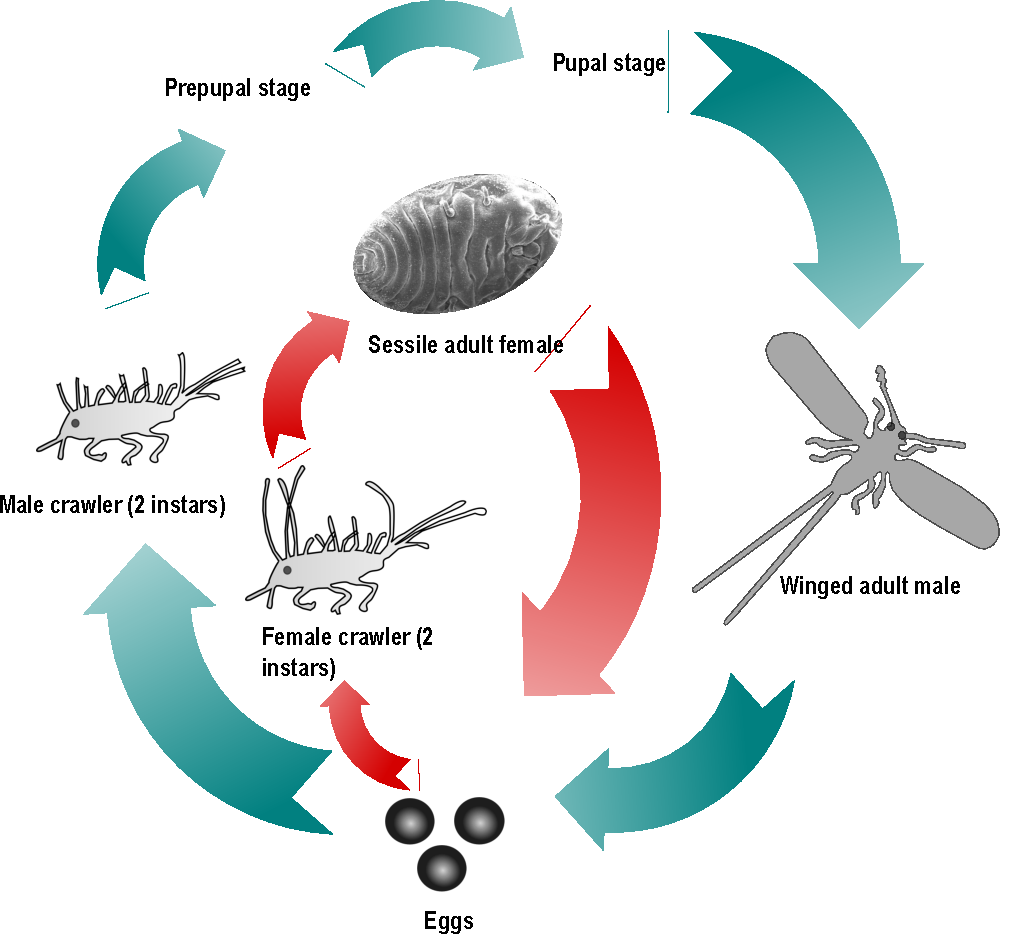
\includegraphics[scale = 0.5]{Images/lifecycle.pdf}
% 	\caption{Lifecycle of \textit{Dactylopius}. Adapted from \citet{Moran1979}}
% 	\label{fig:lifecycle}
% \end{figure}